\section{Shared Memory}
\label{sharedMemory}
The previous chapters introduced the means to enable parallel execution of code in terms of tasks and futures. Still missing from a discussion of ParallelMbeddr's building blocks is the communication between tasks. The communication model of choice for ParallelMbeddr is shared memory. The reason for this choice follows from the objectives for a communication model: it should offer a reasonable performance, considering that it is supposed to be used in embedded systems; it should be reasonably thread-safe by design in order to avoid the trip hazards that are involved with low-level synchronization approaches like mutexes. For performance reasons, transactional memory seems not to be ready for the embedded domain. By following argumentation, for a first communication design, message passing does not offer profound advantages in comparison to shared memory if the access to the shared memory is controlled in a sound way. Usually message passing forbids shared memory between two parallel units of execution. Instead, communication is realized via message sends. A strict separation of memory does not fit the usual C work-flow concerning pointer arithmetic. Therefore, in order to reduce performance losses due to expensive memory copies, some form of memory sharing would have to be introduced into a message passing model. As this would lead to the same problems that already arise with the general shared memory model, the opposite way is chosen: Instead of introducing shared memory in a message passing model, a shared memory model is designed, on top of which message passing can be attached in order to simplify the communication between tasks.\footnote{Such an extension would be a future concern and is not implemented in this work.}

Memory that is to be shared between two tasks must be explicitly declared by an according type. A variable of this type denotes a \textit{shared resource}. Thus, a shared resource can be regarded as a wrapper of data that is to be shared. In order to make use of a shared resource it has to be synchronized first. Specific language elements are used to access and change the value of a shared resource. The chosen approach enables the programmer to use shared data both globally and locally and, like with any other data, nest them inside structs and arrays. Additionally, the new data type enables the IDE to ensure -- despite the (almost) unlimited possibilities to structuring shared resources -- that data are shared in a sound\footnote{`Sound' in this context means `atomic'. Only one task at a time should be able to access a shared datum.} way.

\subsection{Design}
The resources to be shared are typed with the shared resource type:

\begin{equation}
\begin{split}
t & ::= ...|\;\mathit{shared{<}u{>}}\;|\;\mathit{shared{<}shared{<}u{>}{*}{>}}\\
u & ::= t \qquad \textit{void} \neq u \neq t*
\end{split}
\end{equation}

The type parameterization denotes the base type of a shared type, i.e. the type of the data that is wrapped by a shared resource. The base type of a shared resource can be either of mbeddr's C-types, with two exceptions. It must not be \CODE{void} because a shared resource has to wrap an actual value. Furthermore due to reasons that will be explained in \ref{safetyMeasures}, the base type may not denote a pointer to a value that is not shared.\footnote{In other words: A pointer wrapped in a shared resource must point to a shared resource itself. Due to the comprehensive type system that mbeddr is equipped with and that is only partially existent in C99, the compatibility of base types of shared types was mainly tested with the primitive types of C99 as well as pointer types, array types, struct types and type definitions (typedefs). Future work will have to be done to demonstrate and establish full compatibility with the rest of mbeddr's types.} Further restrictions apply to shared types, which are also discussed in \ref{safetyMeasures}. The same applies to the \CODE{.set} expression by which the value of a shared resource can be modified; the value can be retrieved via \CODE{.get}:

\begin{equation}
 e ::= e.\mathit{get}\;|\;e.\mathit{set(e)} 
\end{equation}
\begin{equation}
\inference*[SharedGet]{e |- \mathit{shared{<}t{>}}} {\quad e.\mathit{get} |- t \quad}
\qquad
\inference*[SharedSet]{e |- \mathit{shared{<}t{>}} \quad e' |- t' \quad t' <: t} {\qquad\quad e.\mathit{set}(e') |- \mathit{void} \quad\qquad} 
\end{equation}

In order to access (read or write) the value via \CODE{.get} or \CODE{.set} it must be synchronized first. For this purpose the syntax \texttt{stmts} of statements in mbeddr is extended by the synchronization statement \CODE{sync}. \CODE{sync} contains a \textit{synchronization list} of shared resources to synchronize and a block of statements: % whose referenced shared resources may be synchronized by a surrounding synchronization statement:

\begin{equation}
\mathit{stmt} ::= ...
        |\;\mathit{sync}(res, ..., res) \{\;\mathit{stmt} ... \mathit{stmt}\;\}
\end{equation}
        
\texttt{res} denotes the syntax of possible \textit{synchronization resources}. Each synchronization resource \CODE{res} wraps an expression \CODE{e} which evaluates to a shared resource. \CODE{e} can be either of type \CODE{shared<t>} or of type \CODE{shared<t>*}. A shared resource can be synchronized as it is (as a synchronization resource) or be named (the synchronization resource then becomes a \textit{named resource}):

\begin{equation}
res ::= e\;|\;e\;\mathit{as}\;[\mathit{name}]
\end{equation}

The latter allows the programmer inside the \CODE{sync} statement to refer to the result of an arbitrary complex expression, which evaluates to a shared resource, inside the synchronization statement. Hence, a \textit{named resource} (i.e. a synchronization resource with a name) can be seen as syntactic sugar for a local variable declaration, initialized with a shared resource, and a synchronization resource with a reference thereof. The type of such a reference is given by the shared resource that the expression wrapped by the named resource evaluates to. Due to C's copy semantics, this type is restricted to \CODE{shared<t>*}. This enforcement ensures that the named resource actually synchronizes the original shared resource and not a copy thereof, of which a synchronization would be useless. The scope of a named resource is restricted to the according synchronization statement. More precisely, a named resource \textit{n} of a synchronization statement \textit{s} can be referenced from anywhere inside the abstract syntax tree (AST) of the statement list of \textit{s}. Furthermore, it can be referenced from within the expression of any synchronization resource that follows \textit{n} in the synchronization list of \textit{s}, e.g.:
\begin{ccode}{caption=Synchronization statement with named resources}
shared<shared<int32>> v;
// vContent is declared before it is used in the list => valid
sync(v, &(v.get) as vContent, &vContent->get as vContentContent) {
  vContentContent->set(0);
}
// vContentContent is not in scope, here => invalid
vContentContent->set(1);
\end{ccode}

The introduction of named resources was mainly motivated by the lexical scoping of synchronization resources: In order to determine whether the target of \CODE{.get} or \CODE{.set} is synchronized, ParallelMbeddr checks whether the target is a reference to a visible and synchronized variable or to a named resource. This implies that shared resource expressions other than variable references (e.g. paths and function calls) must be bound by named resources, in order to be able to access their wrapped values via \CODE{.get} or \CODE{.set}. 

In contrast to Java's synchronization blocks and methods \cite[p.~279]{JavaPerformanceTuning}, the synchronization of tasks is not computation oriented, but data oriented. The crucial difference is that a synchronized block \CODE{A} in Java is only protected against simultaneous executions by multiple threads. Thus, it is valid to access the data that are accessed during the execution of \CODE{A} via some other computation whose protecting block (if any) is unrelated to \CODE{A}. Since low-level data races can obviously not be guaranteed to be excluded with this scheme, ParallelMbeddr ties the protection to the data that is to be shared. Every shared resource, i.e. block of shareable data, is therefore protected separately and application-wide. ParallelMbeddr does not yet face higher-level data races, which involve multiple shared resources. Dependencies between shared resources must be resolved by the programmer who has to wrap the dependent data inside a single shared resource, e.g. as fields of a struct. Concluding, if two synchronization blocks, which are about to be executed in parallel, contain synchronization references that overlap in terms of their referenced shared resources, their executions will be serialized. For instance let \textit{t1} and \textit{t2} be two tasks that have access to the same shared resource which is referenced by a global variable \CODE{value}. \textit{t1} wants to synchronize \CODE{value}, simultaneously \textit{t2} wants to synchronize \CODE{valuePointer} which points to \CODE{value}'s shared resource and some other shared resource that is available via the variable \CODE{other}:

\begin{ccode}{caption=Variables that reference equal shared resources}
shared<int32> value;
shared<int32>* valuePointer = &value;
shared<double> other;
\end{ccode}
The synchronization semantics will then cause one thread to wait for the other to finish the execution of the conflicting, and thus blocking, synchronization statement before it starts the execution of its own synchronization statement. The execution order might therefore be changed in the following manner:

\begin{minipage}{1\textwidth}
\adjustbox{valign=t}{
\begin{minipage}{0.4\textwidth}
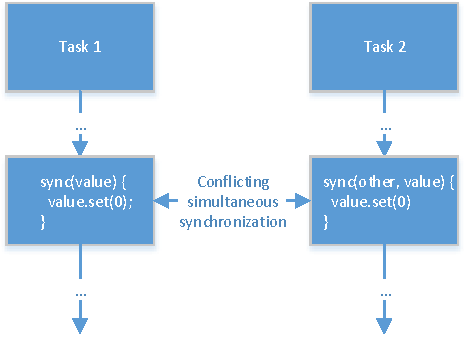
\includegraphics[scale=.9]{pics/ParallelExecutionAttempt}
\end{minipage}
}
\begin{minipage}{0.2\textwidth}
\begin{center}
\vspace{3.5cm}
$\longrightarrow$

actual execution
\end{center}
\end{minipage}
\adjustbox{valign=t}{
\begin{minipage}{0.4\textwidth}
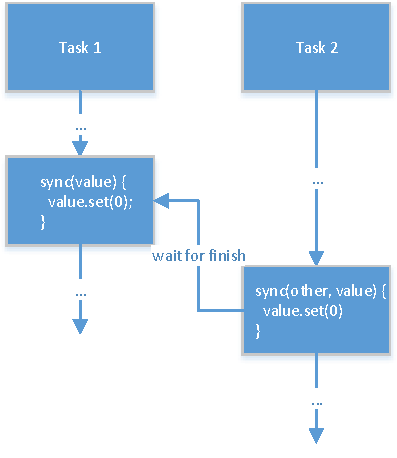
\includegraphics[scale=.9]{pics/SerialExecution}
\end{minipage}}
\captionof{figure}{Serialized execution of conflicting synchronization statements}
\end{minipage}

\vspace*{4mm}

The possibility to refer to multiple shared resources in the synchronization list of a synchronization statement is not mere syntactic sugar for nested synchronization statements. Instead, the semantics of a synchronization list are that all referenced shared resources are synchronized at once, but with a possible time delay. Due to the design of the underlying implementation, deadlocks, as a result of competing synchronization statements, are thus avoided.\footnote{Nevertheless, deadlocks can obviously still occur if nested synchronization statements compete for the same resources in an unsorted order.}

As a result of the fact that generally the access to shared resources is resource-centric, a value wrapped in a shared resource which in turn contains nested shared resources is independently protected from the latter. Therefore, a shared resource of a struct with a shared member \CODE{b} is independently synchronized from \CODE{b}:

%\vspace{0.1cm}
\begin{minipage}{1\textwidth}
\begin{minipage}{0.5\textwidth}
\begin{ccode}{}
struct A {
  int32 a;
  shared<int32> b; 
}
shared<A> sharedA;
shared<int32>* sharedB;
sync(sharedA) { sharedB = &(sharedA.get.b); }
\end{ccode}
\end{minipage}
\begin{minipage}{0.08\textwidth}
\begin{center}
\end{center}
\end{minipage}
\begin{minipage}{0.35\textwidth}
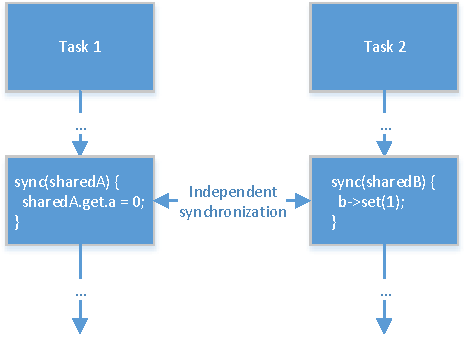
\includegraphics[scale=.9]{pics/ParallelExecution}
\end{minipage}
\captionof{figure}{Parallel execution of non-conflicting synchronization statements}
\end{minipage}

\vspace*{4mm}

For this reason, dependent data should not be separately protected by shared resources, since otherwise data-races could emerge. 

The translation of shared resources is currently only supported for executable programs. Therefore, it is not safe to use shared types and synchronization statements in libraries that are written with mbeddr. The explanations of the following section are thus limited to according scenarios, although the translation for library code would only change in details.

\subsection{Translation of Shared Types}
\label{sharedTypesTranslation}
In order to fully understand the translation of synchronization statements, the translation of shared types is given first. For the implementation of shared types in C, two main solutions are conceivable, which differ in the coupling that they exhibit between the data that is to be shared and the additional data required for access restriction, i.e. synchronization. In any case, a solution must make use of additional data that can be used to synchronize two threads which try to read or write the shared data. To this end, the most basic synchronization primitive was chosen: each protected data item is assigned exactly one mutex. 

In the first solution, the data to be shared is stored as if no protection scheme existed at all. Additionally, all mutexes that are created by the application are stored in one global map, which indexes each mutex by the memory address of its corresponding shared datum. This approach offers the advantage that access to the data itself is not influenced by the mutex protection: Every access \CODE{e.get} of the value of a shared resource  can directly be translated into a reference to the wrapped value. Additionally, since the mutexes are globally managed, all data that is returned by a library can be easily made (pseudo-) synchronization safe. For instance, if a pointer to an arbitrary memory location \texttt{loc} is returned, the pointed-to address can be used to create a new mutex and add a mapping to the global mutex map. However, this on-the-fly protection of memory locations can incur synchronization leaks: The compiler cannot guarantee that address returning functions with unknown implementation will not leak their returned values to some other computation which accesses the according memory unsynchronized. This implies that such protection would only be safe if every reference to \texttt{loc} was wrapped in some shared resource which, in this scenario, is not feasible. Hence, a design was chosen that does not allow for such protection (the interaction with library code is a concern for the future). Consequently, a global map would not be beneficial in this regard. A map solution would entail a space-time trade-off. For instance, Google's C++ \textit{dense\_hash\_map}, \footnote{http://goog-sparsehash.sourceforge.net/doc/dense\_hash\_map.html, accessed: 2014-07-25} provides comparatively fast access to its members but imposes additional memory requirements in comparison to slower hash map implementations\footnote{See http://incise.org/hash-table-benchmarks.html, accessed 2014-07-25, for details. This examplary library should be considered as an illustrative example for the general space-time trade-off that is inherent with maps.}. In spite of their constant time-complexity for accesses, a disadvantage of hash maps is the non-deterministic performance\footnote{Although real-time applications with their time-wise constraints are not a primary concern of this work, it should nevertheless be kept in mind that they are part of the embedded domain. Therefore, a solution that considers the characteristics of this domain for the crucial implementation decisions of ParallelMbeddr is at least regarded advantageous.} and increased access time caused by hash collisions \cite{FastAndDeterministicHashTable}.

The second solution for the implementation of shared types keeps each shareable datum and its mutex together. An instance of a struct with member fields for both components is used in place of the bare datum to be shared. In contrast to the aforementioned solution, a reference to the value \CODE{e.get} needs one level of indirection via the struct instance. However, the access to a mutex is simplified. As with the value, it can be retrieved by a member access to the corresponding struct field, whereas the map solution requires a map lookup to get the mutex (plus additional delay to make any modifying access to the map thread-safe). The computational overhead imposed by a struct member lookup is deemed negligible in the overall application performance. On the other hand, the space required for the struct equals that of the individual fields (value and mutex) plus additional padding \cite[pp.~303 ff.]{LinuxSystemProgramming} that is required to arrange the struct fields along valid memory addresses. The latter depends on the size of the data to be stored. In order to keep the padding as small as possible, smart member ordering should be applied. 

For this work, the struct solution was chosen in order to keep the access time of mutex lookups small and deterministic (except for unforeseeable delays produced by the memory layout) while not imposing too much space and computation overhead for datum lookups. For each kind of shared type \CODE{shared<t>} with the translated base type \CODE{t'} a separate struct is generated:
\begin{ccode}{caption=Struct generated for a shared type}
struct SharedOf_t {
  pthread_mutex_t mutex;
  t' value;
}
\end{ccode}
Any nested shared types are, hence, translated first. For implementation reasons, nested \textit{typedef}s and constants used in array types are also resolved in this process.\footnote{Although the resolution of typedefs and constants impedes corresponding (test-wise) adjustments made by the programmer in the translated C code, this is currently not deemed an issue since, generally, changes should always be made from within mbeddr, i.e. on the original code.} Depending on the base type of the shared type, the generated struct declaration is stored either in a generic module or in a newly generated other module. The following illustration depicts the tree for a type \CODE{shared<t>} whose nodes are made of types and whose edges are formed by the base type relationship of shared types, array types and pointer types,\footnote{Clearly, this tree will have only one branch.} e.g: 


\begin{minipage}{1\textwidth}
\begin{minipage}{0.3\textwidth}
\begin{ccode}{}
struct A { int32 val; }
shared<shared<A[10][20]>*>
\end{ccode}
\end{minipage}
\begin{minipage}{0.4\textwidth}
\begin{center}
\quad$\longrightarrow$\qquad

the simplified type AST
\end{center}
\end{minipage}
\begin{minipage}{0.2\textwidth}
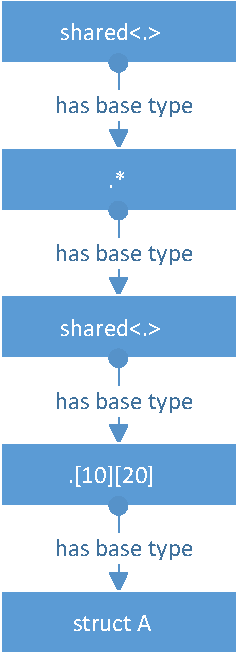
\includegraphics[scale=0.7]{pics/AstForBaseTypes}
\end{minipage}
\captionof{figure}{Abstract syntax tree of a nested shared resource type}
\end{minipage}

\vspace{4mm}
If the leave of the tree is a primitive C type the struct declaration is stored in a generic module. In any other case the leave must be some struct type \CODE{s}. In order to preserve the visibility of the corresponding struct in the newly generated struct \CODE{SharedOf\_t}, the latter is stored in the same module. Since the generation of code related to shared types can diminish the legibility of the resulting code profoundly for every such module, a specific \textit{SharedTypes\_X} module is created and imported into the module that declares \CODE{s}. \textit{SharedTypes\_X} is used to store struct declarations like \CODE{SharedOf\_t}. Furthermore \CODE{s} is lifted into it in order to make it visible in the member declaration \CODE{value} of \CODE{SharedOf\_t}. For any field of \CODE{s} whose type tree contains another user-defined struct type, the corresponding struct declaration is either lifted as well (and recursively treated in the same way), or imported by its module. Should this separation of generated code used for shared type declarations and other user-defined code not proof well in praxis, it could easily be deactivated.
With the former generation of the struct declaration in mind, a type \CODE{shared<t>} is reduced to:
\begin{ccode}{caption=Reduction of a shared resource type}
SharedOf_t
\end{ccode}
The reduction of the expressions \CODE{e.get} and \CODE{e.set(f)} makes use of the \CODE{value} field of the \CODE{SharedOf\_t} struct. The expressions are basically reduced to a retrieval of the field, respectively an assignment to the field:

\vspace{4mm}
\begin{minipage}{1\textwidth}
\begin{minipage}{0.1\textwidth}
\begin{ccode}{}
e'.value
\end{ccode}
\end{minipage}
\begin{minipage}{0.22\textwidth}
\qquad respectively
\end{minipage}
\begin{minipage}{0.15\textwidth}
\begin{ccode}{}
e'.value = f'
\end{ccode}
\end{minipage}
\captionof{lstlisting}{Reductions of \CODE{get} and \CODE{set}}
\end{minipage}
\vspace{0mm}


If \CODE{e'} has a pointer type, the expressions \CODE{e->get} and \CODE{e->set(f)} are reduced to:

\vspace{4mm}
\begin{minipage}{1\textwidth}
\begin{minipage}{0.1\textwidth}
\begin{ccode}{}
e'->value
\end{ccode}
\end{minipage}
\begin{minipage}{0.22\textwidth}
\qquad respectively
\end{minipage}
\begin{minipage}{0.15\textwidth}
\begin{ccode}{}
e'->value = f'
\end{ccode}
\end{minipage}
\captionof{lstlisting}{Reductions of \CODE{get} and \CODE{set} for a pointer}
\end{minipage}
\vspace{0mm}

The mutex of the struct \CODE{SharedOf\_t} in the equally named struct field \CODE{mutex}, which is used to synchronize one variable of an according type, must be initialized prior to any usage. This is done implicitly by generated code, in order to free the programmer from this task. Accordingly, mutexes must be released before they get out of scope to prevent memory leaks. In the generated code, both functionalities make use of corresponding functions, i.e. for every type -- which is one of the following types -- a pair of \CODE{mutexInit}--\CODE{mutexDestroy} functions is generated:

\begin{itemize}
\item shared types whose base types are shared types or for whom mutex functions are recursively generated;
\item array types which are not base types of array types themselves and whose base types are either shared types or struct types for whom mutex functions are recursively generated;
\item struct types whose structs contain at least one field with a type for which the same relation holds as for the aforementioned types.
\end{itemize}

For example, a type \CODE{shared<int32>[42][24]} would enforce the generation of one mutex initialization and one mutex destruction function. \CODE{shared<int32>*} on the other hand would not. Any variable \CODE{v} of the latter type would point to a shared resource which must be referenced directly by another variable \CODE{v'} of type \CODE{shared<int32>} or be contained in the memory-addressable value of some variable \CODE{v''} of a more complex type. The declaration of \CODE{v'}, respectively \CODE{v''}, would then trigger the initialization of the mutex of the shared resource that \CODE{v} points to. The resulting mutex initialization functions for shared types of the aforementioned kind are declared as follows:

\begin{ccode}{caption=Mutex initialization functions}
// for a proper shared type shared<t> and the type t' that t is reduced to
void mutexInit_X(SharedOf_t'* var) { 
  pthread_mutex_init(&var->mutex, &mutexAttribute);
  
  // either if t is a shared type or a struct type:
  mutexInit_X'(&var->value); 
  
  // or if t is an array type t[i_1]...[i_n] of 1 to n dimensions:
  mutexInit_X'((SharedOf_t'*...*)var->value, i_1, ..., i_n); 
}
\end{ccode}
For a shared resource, first the mutex of the corresponding translated struct is initialized by a call to the POSIX function \CODE{pthread\_mutex\_init()}, which takes a mutex pointer and a mutex attribute pointer.\footnote{The meaning of the mutex attribute will be explained later on.} Then -- since by aforementioned conditions the shared resource contains another shared resource -- a call to the appropriate mutex function for the contained value is triggered. Depending on whether the base type of the current shared type is an array, additionally the dimension sizes for this base type may need to be provided as well (see below for details).

For shared ressoures that are nested in arrays, a nested iteration over all elements of the corresponding possibly multidimensional array with calls to either the generated mutex functions or the function defined by the POSIX standard are triggered.

\begin{ccode}{caption=Mutex initialization function for multi-dimensional arrays, label=arrayMutexInit}
// for a proper array type t[]...[] of 1 to n dimensions where '...' denotes the occurrence of 
// an according number of symbols and t' denotes the reduced-to type
void mutexInit_X(t'*...* var, int32 size_0, ..., int32 size_n) { 
  for (int32 __i_0 = 0; __i_0 < size_0; __i_0++) { 
    ...
      for (int32 __i_n = 0; __i_n < size_n; __i_n++) {
        // in case t is a struct type
        mutexInit_X'(&var[__i_0]...[__i_n]);
        
        // or, in case t is a shared type with generic C base type:
        pthread_mutex_init(&var[__i_0]...[__i_n].mutex, &mutexAttribute);
      }
    ...
  } 
}
\end{ccode}

For structs with nested shared resources, for each field that is or contains a shared resource, either the \CODE{pthread\_mutex\_init()} function is called directly or the mutex initialization is done by a call to the already generated function that is type compatible with this field (by possibly providing additional array dimensions):

\begin{ccode}{caption=Mutex initialization function for structs}
// for a proper struct type t of a struct t { u_1 f_1; ...; u_n f_n } and according reduced 
// field types u_1' to u_n'
void mutexInit_X(SharedOf_t* var) {
  ...
  // if u_i demands further initialization and it is a struct type or a shared type
  mutexInit_X'(&var->f_i);
  
  // if u_i demands further initialization and is an array type u_i[j_1]...[j_n] of 1 to n dim.
  mutexInit_X'((SharedOf_u_i'*...*)var->f_i, j_1, ..., j_n);
  
  // or, if u_i is a shared type with a generic C base type:
  pthread_mutex_init(&var->f_i.mutex, &mutexAttribute);
  ...
}
\end{ccode}
The signature of \CODE{mutexInit\_X()} for arrays in line 3 of listing \ref{arrayMutexInit} shows that those are not passed as arrays to the mutex functions, but as pointers. This is due to the necessity of declaring multidimensional arrays at least partially with the size for each dimension (e.g. \CODE{int[][]} would be missing at least one dimension size). Nevertheless it would not make sense to declare one mutex function for each shape of dimension size. Since arrays are treated like pointers internally when they are passed as function arguments, it is completely safe to cast them to appropriate pointer types and to use equal types for the according function parameters.

The deletion of mutexes is defined quite similar to the initialization, with the main difference that the utilized according pthreads function only takes one mutex. Therefore, only the deletion of mutexes nested in resources of shared types is shown:
\begin{ccode}{caption=Mutex destruction function}
void mutexDestroy_X(SharedOf_t'* var) { 
  pthread_mutex_destroy (&var->mutex); 
  // ... further call to a mutexDestroy_X function equivalent to mutexInit_X shown above
}
\end{ccode}
The presented functions are used to initialize mutexes at the beginning of their life span and delete them right before the corresponding end. For mutexes referred to by global variables this means that they must be initialized at the beginning of the entry function of the program.\footnote{Due to the way mutexes are used in ParallelMbeddr (recursively and nested in structs -- as will be shown in the following paragraphs) and the peculiarities of C and the POSIX standard, there is no way to combine the definition and the initialization of mutexes.} As already forced for executable programs by mbeddr, the programmer thus has to specify a main function (the construction of libraries is not supported by ParallelMbeddr, yet). Similarly, mutexes of local variables are initialized right after their declaration, whereas mutexes of function arguments are declared at the beginning of the related function.\footnote{\label{mutexCopies}It is not an obvious choice to enable the programmer to use function arguments of shared resources: C's pass-by-value semantics of function parameters causes parameters to be copied into functions. Therefore, a shared resource which is not passed by its address but by its actual value will provoke the generation of another, equal shared resource at the beginning of the function execution. This copy is synchronization-wise completely unrelated to the original shared resource, since mutex copies cannot be used to lock with their origins \cite{Mutexes}. Furthermore, they have to be initialized and destroyed separately. The use of shared resources in such a manner can confuse programmers who are not aware of this fact. Nevertheless, ParallelMbeddr allows this kind of utilization of shared resources in order to not burden the programmer with having to copy large structs that contain shared resources component-wise if the shared resource data is not of relevance. Depending on the feedback of future users, it should be considered whether warnings for unintended misuse of shared resources in this way might be helpful.} The deletion of mutexes for shared resources must be accomplished before they get out of scope which, again, depends on the kind of variables they are referred to. 

Mutexes for global variables need not be destroyed at all in order to avoid memory leaks. Their lifetimes span the whole program execution so that the  memory allocated to these mutexes will be cleaned up by the operating system. On the other hand, the mutexes of local variables must be destroyed before they get out of scope. Hence, mutex destruction calls are added at the end of the surrounding scopes of mutexes. If control flow breaking statements (\textit{return}, \textit{break}, \textit{continue}, \textit{goto}) are present, additional calls are inserted according to the following rules. Let \textit{c} denote a control-flow-breaking statement that occurs in the AST of the same function as the declaration \textit{l} of some local variable, which refers to a (nested) shared resource. If \textit{c} is part of the AST of any statement that follows \textit{l}\footnote{In other words, only those control-flow-breaking statements \textit{c}s that are either one of the statements \textit{stmt}s which have the same AST parent \textit{p} and follow \textit{l} in the statement list of \textit{p} or are contained in the AST of some \text{stmt} are considered.} and
\begin{itemize}
\item \textit{c} is a \textit{return} statement and refers to a function or a closure whose AST contains \textit{l} or
\item \textit{c} is a \textit{break} statement and refers to a loop or a \textit{switch} statement case whose AST contains \textit{l} or
\item \textit{c} is a \textit{continue} statement and refers to a loop whose AST contains \textit{l} or
\item \textit{c} is a \textit{goto} statement and refers to a label outside the AST of any statement that follows \textit{l},\footnote{Since \textit{goto} statements can considerably disorganize the program flow they should be only used with great care in ParallelMbeddr. Specifically the initialization of mutexes is not protected against misuse of these statements.}
\end{itemize}
\textit{c} must be preceded with a destruction call of the mutex of the shared resource of \textit{l} (compare with the synchronization stopping rules below). Allocated memory that is not freed at the end of the program is automatically released by the operating system. Hence, a \textit{return} statement that refers to the entry function of the program need not be preceded with destruction calls of its local shared resources. The proper destruction of a mutex of an argument of function \textit{f} just requires according function calls at the end of \textit{f} and before any return statement that refers to \textit{f}. 

Like inside the declarations of the mutex initialization functions explained above, the actual initialization function to call for a variable or argument is either one of the \CODE{mutexInit\_X()} functions or a direct call of \CODE{pthread\_mutex\_init()} for `simple' shared resources of generic C types, e.g.:\footnote{The same reasoning holds for calls of mutex destruction functions.}

\vspace{4mm}
\begin{minipage}{1\textwidth}
\begin{center}
\begin{minipage}{0.3\textwidth}
\begin{ccode}{}
// simple shared resource
shared<int32> v1;

// complex shared resource
shared<int32>[2][3] v2;
\end{ccode}
\end{minipage}
\qquad$\Longrightarrow$\qquad\qquad
\begin{minipage}{0.5\textwidth}
\begin{ccode}{}
SharedOf_int32_0 v1;
pthread_mutex_init(&v1.mutex, &mutexAttribute);

SharedOf_int32_0[2][3] v2;
mutexInit_0((SharedOf_int32_0**)v2, 2, 3);
\end{ccode}
\end{minipage}
\end{center}
\captionof{lstlisting}{Mutex initialization calls for local variables}
\end{minipage}
\vspace{4mm}

To recap: The mutex of a shared resource is either directly initialized and destroyed via appropriate pthreads functions or it is indirectly handled via functions that are based on the types of the values that shared resources are nested in. This approach was chosen in order to reduce the amount of code duplication that would occur if mutexes of shared resources would be handled inline for every according variable. As a result, the generated code's readability is enhanced. The additional computational overhead due to function calls and returns should be regarded as an optimization concern of a further compilation step by a compiler like \textit{gcc}.

ParallelMbeddr does not prevent the programmer from structuring the synchronization statements in such a way that a task will synchronize a variable of a shared resource multiple times (\textit{recursive synchronization}). The following code depicts such behavior:
\begin{ccode}{caption=Recursive synchronization}
shared<int32> sharedValue;
sync(sharedValue) {
  sync(sharedValue) {
    sharedValue.set(42);
  }
}
\end{ccode}
Since each synchronization statement locks the mutexes of the referred shared resources (see below for details), a recursive synchronization results in a \textit{recursive lock} of the corresponding mutex. Mutexes as defined by the POSIX standard must be specifically initialized in order to allow for this behavior:\footnote{By default, a recursive lock results in undefined behaviour because a default mutex does not have a lock count which is required to make recursive locks work: http://linux.die.net/man/3/pthread\_mutex\_trylock, accessed: 2014-07-28.} A mutex attribute that specifies the recursiveness must be defined and initialized first. It can then be used by any number of mutexes. For this purpose, an application-wide attribute is defined in a generic module that is imported by all user-defined modules. It is initialized at the beginning of the main function:

\vspace{10mm}
\begin{ccode}{caption=Global mutex attribute for recursive mutexes}
// inside the generic module:
pthread_mutexattr_t mutexAttribute
// at the beginning of main:
pthread_mutexattr_init(&mutexAttribute);
pthread_mutexattr_settype(&mutexAttribute, PTHREAD_MUTEX_RECURSIVE);
\end{ccode}

\subsection{Translation of Synchronization Statements}
Every synchronization statement is reduced to its statement list -- as a block --, surrounded with calls to functions that control the synchronization of the mutexes. The reduction of such a statement is given either by

\vspace{4mm}
\begin{minipage}{1\textwidth}
\begin{center}
\begin{minipage}{0.31\textwidth}
\begin{ccode}{}
sync(e) stmt_list
\end{ccode}
\end{minipage}
\qquad$\Longrightarrow$\qquad\quad
\begin{minipage}{0.5\textwidth}
\begin{ccode}{}
startSyncFor1Mutex(&e.mutex);
stmt_list'
stopSyncFor1Mutex(&e.mutex);
\end{ccode}
\end{minipage}
\end{center}
\captionof{lstlisting}{Reduction of a synchronization statement}
\end{minipage}
\vspace{2mm}

in case it contains only one synchronized resource, or else by

\vspace{4mm}
\begin{minipage}{1\textwidth}
\begin{center}
\begin{minipage}{0.31\textwidth}
\begin{ccode}{}
sync(e_1, ..., e_n) stmt_list
\end{ccode}
\end{minipage}
\quad$\Longrightarrow$\quad\quad
\begin{minipage}{0.53\textwidth}
\begin{ccode}{}
startSyncForNMutexes(&e_1.mutex, ..., &e_n.mutex);
stmt_list'
stopSyncForNMutexes(&e_1.mutex, ..., &e_n.mutex);
\end{ccode}
\end{minipage}
\end{center}
\captionof{lstlisting}{Reduction of a synchronization statement with multiple synchronization resources}
\end{minipage}
\vspace{2mm}

The statements are kept inside their statement list block in order to preserve the scope of local variables inside synchronization statements. A synchronization statement list block is reduced to another block where each statements that breaks the program flow structure may be preceded by an identical call of the \CODE{stopSyncForNMutexes()} function as in line 3: Let \textit{s} be a synchronization statement and \textit{c} be a control-flow-breaking statement which is nested in the AST of \textit{s}' statement list. Then \textit{c} is preceded with a call to \CODE{stopSyncForNMutexes()} if one of the following cases holds:
\begin{itemize}
\item \textit{c} is a \textit{return} statement and refers to a function or a closure whose AST contains \textit{s};
\item \textit{c} is a \textit{break} statement and refers to a loop or a \textit{switch} statement case whose AST contains \textit{s};
\item \textit{c} is a \textit{continue} statement and refers to a loop whose AST contains \textit{s};
\item \textit{c} is a \textit{goto} statement and refers to a label outside the AST of \textit{s}.\footnote{Similarly to the aforementioned problem with mutex management functions, \textit{goto} statements can impair synchronization states and should therefore be used with great care. This holds particularly for \textit{goto} statements which cause jumps into synchronization statements from outside.}
\end{itemize}

In this manner, inconsistent synchronization states of shared resources due to a control flow break by the aforementioned statements are omitted. Since the occurrence of such a statement may also force ParallelMbeddr to insert \CODE{mutexDestroy\_X()} calls, a careless mixture of mutex unlocking and destruction calls can cause runtime errors \cite{Mutexes}. The generator therefore ensures that any destruction calls are put behind the generated unlocking calls.

For each arity of synchronization resources, separate versions of the \CODE{start}- and \CODE{stopSyncForNMutexes()} functions are declared inside a generic C module. A \CODE{stopSyncForNMutexes()} function straightforwardly redirects its mutex parameters to calls of the \CODE{pthread\_mutex\_unlock} function:
\begin{ccode}{caption=Synchronization stopping function}
// the corresponding function 'stopSyncFor1Mutex()' for exactly one mutex is skipped here
void stopSyncForNMutexes(pthread_mutex_t* mutex_1, ..., pthread_mutex_t* mutex_n) { 
  pthread_mutex_unlock (mutex_1);
  ...
  pthread_mutex_unlock (mutex_n); 
}
\end{ccode}

Abstracted from the details of the actual implementation, synchronization statements synchronize their resources atomically, as was mentioned in the preceding design section. Since one or more mutexes can be tentatively locked by multiple threads simultaneously, specific contention management has to be conducted. The illusion of atomic synchronization is realized by an implementation of the obstruction-free\footnote{Busy-waiting means that the thread will repeatedly test a condition until it is met, without doing actual useful work \cite[p.~166]{AnIntroductionToParallelProgramming}. Thus, it is an alternative to suspending a thread and revoking it later on when some condition is met (which can, e.g., be realized by \textit{condition variables} as provided by POSIX threads \cite[p.~77]{ProgrammingWithPOSIXThreads}). Obstruction-free means that the execution of any thread will progress when at some time the thread is run in isolation, i.e. when the execution of obstructing other threads is interrupted meanwhile. The existence of obstruction-freedom guarantees that no deadlocks will occur \cite{ObstructionFreeAuthorizationEnforcement}. However, livelocks and starvation are not necessarily avoided. Stronger degrees of non-blocking algorithms like lock-freedom and wait-freedom tackle these problems (partially), but are not relevant for this work. Further information on the latter is for instance provided by http://preshing.com/20120612/an-introduction-to-lock-free-programming/, accessed: 2014-07-28.} busy-wait protocol \textit{Polite}. In order to resolve conflicts, \textit{Polite} uses exponential back-off. The according back-off function is explained further down. The synchronization function tries to lock every mutex as given by its arguments. On failure, it releases every mutex that was locked so far, uses the back-off function to delay its execution for a randomized amount of time, and repeats afterwards. This scheme enables competing threads to (partially) proceed and avoid deadlocks due to unordered overlapping mutex locks.\footnote{Again, the presented scheme does not prevent the programmer from nesting the synchronization statements in such a manner that deadlocks in nested synchronization statements occur. It is rather a prevention of deadlocks that are caused solely by synchronization statements on the same nesting level.}
\begin{ccode}{caption=Synchronization starting function}
// again, the equivalent function declaration for one mutex is skipped
void startSyncForNMutexes(pthread_mutex_t* mutex_0, ..., 
                          pthread_mutex_t* mutex_m, pthread_mutex_t* mutex_n) { 
  uint8 waitingCounter = 0; 
  uint16 mask = 16; 
  uint32 seed = (uint32)(uintptr_t) &waitingCounter;
  
  while (true) { 
    if ([| pthread_mutex_trylock (mutex_0) |] != 0) { 
      backoffExponentially(&waitingCounter, &mask, &seed); 
    } 
    else if ([| pthread_mutex_trylock (mutex_1) |] != 0) { 
      [| pthread_mutex_unlock (mutex_0) |]; 
      backoffExponentially(&waitingCounter, &mask, &seed); 
    } ...
    else if ([| pthread_mutex_trylock (mutex_n) |] != 0) { 
      [| pthread_mutex_unlock (mutex_m) |];
      ...
      [| pthread_mutex_unlock (mutex_0) |]; 
      backoffExponentially(&waitingCounter, &mask, &seed); 
    } 
    else { break; }
  }
}
\end{ccode}

The back-off realized by Polite delays the execution  by less than \textit{limit} $ = 2^{n+k}$ ns \cite{AdvancedContentionManagement} in a randomized fashion. \textit{n} denotes the retry counter and \textit{k} denotes some constant offset which can be machine-tuned. The randomized wait time of the exponential back-off is used to avoid livelocks which could happen if two threads would repeatedly compete for the same resources and delay their execution for equal amounts of time. In the current implementation \CODE{backoffExponentially()} of the contention management, the offset \textit{k} is set to 4 and a threshold \textit{m} of 17 denotes the number of rounds after which \textit{k} is reset.\footnote{\textit{k}'s value is reflected in the initial value ($2^4 = 16$) of \CODE{mask} whereas \textit{m}'s value is composed of mask's base and the divisor (13) in the calculation of the next \CODE{waitingCounter}.} Thus, maximum delays of about 100 ms (specifically 131 ms) are allowed.\footnote{The search for machine- or application-specific optimal offsets and thresholds is a task for future enhancements of ParallelMbeddr.}
\begin{ccode}{caption=Exponential back-off function}
inline void backoffExponentially(uint8* waitingCounter, uint16* mask, uint32* seed) { 
  *mask |= 1 << *waitingCounter; 
  randomWithXorShift(seed); 
  struct timespec sleepingTime = (struct timespec){ .tv_nsec = *seed & *mask }; 
  nanosleep(&sleepingTime, null); 
  *waitingCounter = (*waitingCounter + 1) % 13; 
}
\end{ccode}
It has to be noted that \CODE{backoffExponentially()} keeps its main state inside the \CODE{startSyncForNMutexes()} function. The state will therefore be re-initialized before the execution of every synchronization block. The generation of the pseudo-randomized delay is realized via utilization of the Marsaglia's Xorshift random number generator \cite{XorshiftRngs}:
\begin{ccode}{caption=Pseudo randomization via Xorshift}
void randomWithXorShift(uint32* seed) { 
  *seed ^= *seed << 13; 
  *seed ^= *seed >> 17; 
  *seed ^= *seed << 5; 
}
\end{ccode}
The generator was chosen for its high performance, low memory consumption, and thread-safety due to the utilization of the \CODE{seed} parameter which points to a stack-managed local variable as opposed to the global state usage of the standard C random generator \CODE{rand()}. The fact that after a certain number -- which may be smaller than in other generators -- of repeated calls with the same seed value, repetitions of the sequence of calculated numbers will occur is not of relevance for the purpose of this work.

\subsection{Example Code}
\label{sharedMemoryExample}
In the previous sections \ref{taskExample} and \ref{futuresExample} the running example approximated the number $\pi$ by using tasks which calculate exactly one fraction of the result each and by retrieving their results via futures. The amount of work was therefore partitioned in advance. In this section, a more dynamic approach is chosen instead: The logic of every task comprises major and minor rounds. A minor round is equivalent to the full calculation loop in the previous $\pi$ solution. In every step of a major round, a minor round is initiated by first coordinating with the other tasks which range of $\pi$ the current task should calculate. After having calculated the sum in a minor round, the task then uses a queue to store its next partial result. A dedicated task is used to collect these partial results from the queue and accumulate them to a complete sum, which eventually becomes the result of the over-all approximated $\pi$. The communication-based solution can be seen as a map-reduce implementation where partial results are mapped onto the queue by a certain number of tasks and from there reduced to a final result by a separate task (compare with \cite{MapReduce}).
In order to understand the new implementation, the following example is given: A thread-safe queue of type \CODE{long double} with a certain number of slots is to be viewed as a black box. Further, it has to be supposed that functions for the initialization, for adding a value and getting the next value (or wait for the next value), exist:
\begin{ccode}{caption=Function definitions for the queue}
struct Queue {...}
void queueInit(shared<Queue>* queue);
void queueSafeAdd(shared<Queue>* queue, long double item);
void queueSafeGet(shared<Queue>* queue, long double* result);
\end{ccode}
As in the previous approach, the amount of work to be done is defined by a range size (number of minor task rounds) and the number of ranges altogether. Additionally, the number of mapper tasks is set to a certain value that should be in the order of the number of processor cores:
\begin{ccode}{}
#constant BLOCKSIZE = 300000000; 
#constant BLOCKCOUNT = 4; 
#constant THRESHOLD = BLOCKSIZE * BLOCKCOUNT; 
#constant MAPPERCOUNT = 2;
\end{ccode}
These constants are used to initialize the mappers and the reducer in the main function appropriately:
\begin{ccode}{caption=Initialization of the mappers and the reducer}
exported int32 main(int32 argc, string[] argv) { 
  shared<Queue> queue; 
  queueInit(&queue); 
  shared<Queue>* queuePointer = &queue; 
   
  shared<uint32> counter; 
  shared<uint32>* counterPointer = &counter; 
  sync(counter) { counter.set(0); } 

  Task<void> mapperTask = |map(THRESHOLD, counterPointer, queuePointer)|; 
  Future<void>[MAPPERCOUNT] mappers; 
  for (i ++ in [0..MAPPERCOUNT[) { 
    mappers[i] = mapperTask.run; 
  }
  mapperTask.clear;
   
  shared<long double> result; 
  shared<long double>* resultPointer = &result; 
   
  |reduce(BLOCKCOUNT, resultPointer, queuePointer)|.run.join;
  
  return 0; 
}
\end{ccode}

First, the queue is defined as being shared in order to be accessible by all tasks. After the initialization, a pointer to the queue is created, which is necessary since any other reference inside a task expression to the queue variable would otherwise cause a copy of the queue struct instance into the task, regardless of whether later on the address of the referred value is retrieved via the \CODE{\&} operator. This `shortcoming' of the current semantics could be addressed by the introduction of a new address operator that creates a temporary variable of the addressed value and should be considered for future extensions of ParallelMbeddr. Similar to the queue, a \CODE{counter} variable is introduced which will be used by the tasks to check and communicate how many blocks have been processed so far. Then, one mapper task is defined and initialized with a task expression of a call to the \CODE{map()} function. For communication purposes, the mapper gets the queue pointer and the counter pointer. Additionally, although due to the use of constants not necessary in the current example, the mapper task is told the maximum number of items that need to be calculated. This single task template\footnote{\CODE{mapperTask} can be seen as a template for actual running mapper task instances.} is used to create multiple running tasks and store their handles as futures in a \CODE{mappers} array. The reducer uses a pointer to the memory location of \CODE{result} to store its result. Furthermore, it gets access to the queue via a pointer thereof and is told how many items (\CODE{BLOCKCOUNT}) it shall read from the queue before termination. In line 20, the code shows the first example of a task expression chain: First the task is declared, then an instance of it is run in parallel and immediately the main task joins the reducer. Since nothing is done in the main task between the run and the join, the serialized execution could also be realized by a simple function call to \CODE{reduce()}. For demonstrative purposes, the code was chosen this way nevertheless. The main task solely joins the reducer task, since after its termination every mapper task will also be finished.
The \CODE{map()} function iteratively calculates complete ranges (blocks) of fractions of $\pi$ until the maximum number of items, as given by \CODE{threshold}, is reached:
\begin{ccode}{caption=Mapper function}
void map(uint32 threshold, shared<uint32>* counter, shared<Queue>* resultQueue) { 
  while (true) { 
    uint32 start; 
    uint32 end; 
     
    sync(counter) { 
      start = counter->get; 
      if (start == threshold) { 
        break; 
      } 
      uint32 possibleEnd = start + BLOCKSIZE; 
      end = (possibleEnd <= threshold)?(possibleEnd):(threshold); 
      counter->set(end); 
    } 
     
    queueSafeAdd(resultQueue, calcPiBlock(start, end)); 
  } 
}
\end{ccode}
In every iteration, the function synchronizes the shared resources that \CODE{counter} points to in order to retrieve its value and increment it by the number of items that \CODE{map()} is going to calculate in the current round. It uses the \CODE{calcPiBlock()} function that was presented in section \ref{taskExample} to calculate a partial sum. Afterwards, the result is added to the queue. 
The \CODE{reduce()} function uses the queue to iteratively read all partial results and update the value of the shared resource of the final result accordingly:
\begin{ccode}{caption=Reducer function}
void reduce(uint32 numberOfItems, shared<long double>* finalResult, 
            shared<Queue>* partialResultQueue) {
  sync(finalResult) { 
    for (uint32 i = 0; i < numberOfItems; ++i) { 
      long double item; 
      queueSafeGet(partialResultQueue, &item); 
      finalResult->set(item + finalResult->get); 
    }
  }
}
\end{ccode}
During the whole calculation, \CODE{reduce()} synchronizes the result in order to keep the overall synchronization overhead small. It is able to do this because no other task will try to access the result before the termination of the single reducer task.

In the beginning of the translated main function, the global mutex attribute, which will be reused for every mutex, is initialized. Afterwards, the declared queue is initialized:
\begin{ccode}{caption=Reduction of the queue variable inside the main function}
pthread_mutexattr_settype(&mutexAttribute_0, PTHREAD_MUTEX_RECURSIVE); 
pthread_mutexattr_init(&mutexAttribute_0); 
initAllGlobalMutexes_0(); 
SharedOf_Queue_0 queue; 
mutexInit_2(&queue); 
queueInit(&queue); 
SharedOf_Queue_0* queuePointer = &queue;
\end{ccode}
The translated struct type \CODE{SharedOf\_Queue\_0} of the original type \CODE{shared<Queue>} denotes a struct that contains a field for the protected queue and a mutex field:
\begin{ccode}{caption=Reduction of the queue's type}
struct SharedOf_Queue_0 { 
  pthread_mutex_t mutex; 
  Queue value; 
};
\end{ccode}
The mutex initialization function \CODE{mutexInit\_2()} initializes the mutex of the shared queue and calls another initialization function which, in turn, initializes any nested mutexes of the \CODE{Queue} struct. Similarly, a destruction function is generated:
\begin{ccode}{caption=Mutex management functions for type \CODE{shared<Queue>}}
void mutexInit_2(SharedOf_Queue_0* var) { 
  pthread_mutex_init(&var->mutex, &mutexAttribute_0); 
  mutexInit_1(&var->value); 
}
void mutexDestroy_2(SharedOf_Queue_0* var) { 
  pthread_mutex_destroy(&var->mutex);
  mutexDestroy_1(&var->value); 
}      
\end{ccode}
Similar to the declarations for the queue, the mbeddr generator creates declarations of a struct for the \CODE{result} variable. The initialization and destruction of \CODE{result} is accomplished inline by calls to the pthreads functions, since no nested mutexes for the fields of the struct exist:
\begin{ccode}{caption=Reduction of the \CODE{result} variable}
struct SharedOf_long_double_0 { 
  pthread_mutex_t mutex; 
  long double value; 
};
... // in main()
SharedOf_long_double_0 result; 
pthread_mutex_init(&result.mutex, &mutexAttribute_0); 
SharedOf_long_double_0* resultPointer = &result;
\end{ccode}
Lastly, the \CODE{counter} variable shows how translated shared resources can be synchronized.\footnote{The declarations of the struct and the mutex functions for the \CODE{counter} variable are skipped.} For the duration of the setting of \CODE{counter}'s value, its mutex is locked. The setting of the value is done by an assignment to the \CODE{value} field of the generated struct that keeps the value of the shared resource:
\begin{ccode}{caption=Reduction of the \CODE{counter} variable}
SharedOf_uint32_0 counter; 
pthread_mutex_init(&counter.mutex, &mutexAttribute_0); 
SharedOf_uint32_0* counterPointer = &counter;

startSyncFor1Mutex(&counter.mutex); 
{ counter.value = 0; } 
stopSyncFor1Mutex(&counter.mutex);
\end{ccode}

The mutexes of all shared resources are destroyed at the end of the main function. Although this should not be necessary for local variables of the entry function of the program, the compiler currently does not distinguish between the main function and any other function for which such calls would be necessary:
\begin{ccode}{caption=Mutex destructions at the end of the main function}
mutexDestroy_2(&queue); 
pthread_mutex_destroy(&counter.mutex); 
pthread_mutex_destroy(&result.mutex);
\end{ccode}
The initializations of the tasks and the declarations of the futures are quite similar to those in section \ref{taskExample}:
\begin{ccode}{caption=Reductions of tasks and futures, label=lst:taskFutureReduction}
Task mapperTask = taskInit_0(queuePointer, counterPointer);
// mappers:
VoidFuture[MAPPERCOUNT] mappers; 
for (int8 __i = 0; __i < MAPPERCOUNT; __i++) { 
  mappers[__i] = runTaskAndGetVoidFuture(mapperTask); 
}
free(mapperTask.args);

// reducer:
saveAndJoinVoidFuture(futureInit_0(resultPointer, queuePointer));
\end{ccode}

Since in the new solution, the tasks do not return any results directly, the \CODE{VoidFuture} struct and respective functions are used.\footnote{As the declarations of the \CODE{taskInit\_0()} function and the \CODE{Args\_X} structs resemble equivalent declarations of previously discussed code examples they are skipped here.} The reduction of the original code \CODE{|reduce(RANGECOUNT, resultPointer, queuePointer)|.run.join} to the code in line 10 of listing \ref{lst:taskFutureReduction} is done in the following manner. As was shown in section \ref{futuresTranslation}, the \CODE{run} call and the task declaration are reduced to a call of a function which combines the initialization of a task with the one of a future of a parallel running instance of this task. This call is reflected by \CODE{futureInit\_0(resultPointer, queuePointer)}. Furthermore, the join of the task must first bind the created future handle to some addressable location before it can use this handle by its address. For this reason \CODE{saveAndJoinVoidFuture} is used in place of \CODE{joinVoidFuture}. The declaration of \CODE{futureInit\_0} follows:
\vspace{4mm}
\begin{ccode}{caption=Future initialization function generated for the queue}
VoidFuture futureInit_0(SharedOf_long_double_0* resultPointer, SharedOf_Queue_0* queuePointer) { 
  Args_1* args_1 = malloc(sizeof(Args_1)); 
  args_1->resultPointer = resultPointer; 
  args_1->queuePointer = queuePointer; 
  pthread_t pth; 
  pthread_create (&pth, null, :parFun_1, args_1) |]; 
  return (VoidFuture){ .pth = pth }; 
}
\end{ccode}
The original declaration of the reducer task contains references to the local variables \CODE{resultPointer} and \CODE{queuePointer}, which is why they are bound to equally named fields in the argument struct. An instance of the \CODE{VoidFuture} struct is returned because the parallel task does not return a value and, thus, has the type \CODE{task<void>}.

Inside the helper function \CODE{map()}, the synchronization statement of \CODE{counter} is replaced by its statement list, which is surrounded by calls to appropriate functions:
\begin{ccode}{caption=Reduction of the synchronization statement inside \CODE{map()}}
while (true) {
  uint32 start; 
  uint32 end;
  
  startSyncFor1Mutex(&counter->mutex); 
  { 
    start = counter->value; 
    if (start == threshold) { 
      stopSyncFor1Mutex(&counter->mutex); 
      break; 
    }
    uint32 possibleEnd = start + BLOCKSIZE; 
    end = (possibleEnd <= threshold)?(possibleEnd):(threshold); 
    counter->value = end; 
  } 
  stopSyncFor1Mutex(&counter->mutex);
  
  queueSafeAdd(resultQueue, calcPiBlock(start, end));
}
\end{ccode}
The break statement in line 10 is preceded by another call to the synchronization stop function, as the function would otherwise return in a state where \CODE{counter} would still be locked, which would ultimately cause the program to fail. The former expressions to get and set the value of \CODE{counter} are translated into accesses of the translated \CODE{value} field of the \CODE{counter} struct instance. The synchronization statement of \CODE{reduce()} is likewise translated into its statement list with surrounding synchronization calls. In line 6, the translation of the expression \CODE{finalResult->set(item + finalResult->get)} contains two accesses to the aforementioned \CODE{value} field, one for \CODE{.set} and one for \CODE{.get}:
\begin{ccode}{caption=Reduction of the synchronization statement inside \CODE{reduce()}}
startSyncFor1Mutex(&result->mutex); 
{ 
  for (uint32 i = 0; i < numberOfItems; ++i) { 
    long double item; 
    queueSafeGet(resultQueue, &item); 
    result->value = item + result->value; 
  }
} 
stopSyncFor1Mutex(&result->mutex);
\end{ccode}
